\section{Experimental Setup}
\label{sec:setup}

\textbf{Corpus.} We generate a synthetic entity-question corpus in the
spirit of controlled knowledge-store studies \citep{allen2023physics}: a
vocabulary of $1{,}600$ invented entities, each assigned to generated
questions with deterministic single-token-friendly answers. The
memorization split $\mathcal{D}_{\mathrm{mem}}$ contains 1{,}200
examples in a fixed template with an \texttt{Answer:} suffix; the
generalization split $\mathcal{D}_{\mathrm{gen}}$ (450 prompts) asks the
same facts through paraphrase and chaining templates never seen in
training, so exact match on it measures \emph{use} rather than recall.
Dataset construction details and templates are in
Appendix~\ref{app:dataset}.

\textbf{Models and training.} We train Qwen2.5-0.5B-Instruct and
Qwen2.5-7B-Instruct \citep{qwen2024qwen25} with LoRA
($r{=}16$, $\alpha{=}32$, dropout $0.05$) on all attention and MLP
projections, probe layer $l^\star{=}12$ and $l^\star{=}14$
respectively, backbone LR $2{\times}10^{-5}$ (cosine, $10\%$ warmup),
effective batch 16, probe LR $10^{-3}$, gate parameters
$\tau_0{=}0.8$, $\delta_0{=}0.1$, $\lambda_0{=}0.3$, and the controller
of Section~\ref{sec:method:control} with $m_{\min}{=}0.5$. Each model
trains for up to 50 epochs (75 steps/epoch) on a single H100 in bf16;
the 0.5B run completed all 50 epochs (3{,}750 steps), while the 7B run
was terminated by compute-budget exhaustion during epoch 28, after 27
completed epochs with the gate open. All telemetry---per-epoch gate
evaluations, controller decisions, probe states, matrices, and the
complete stdout logs---is persisted to the Hugging Face Hub
(Appendix~\ref{app:artifacts}).

\textbf{Metrics.} Each epoch we log: likelihood recall $\amemlf$
\eqref{eq:lf}; token-level recall; free-generation exact match
$\amemem$; substring containment of the target in the generation;
paraphrase exact match $\agen$; the probe's accuracy on memorized vs.\
held-out entity states; mean training loss; and held-out eval loss.
Table~\ref{tab:main} summarizes the endpoints of both runs.

\begin{table}[t]
\centering
\small
\begin{tabular*}{\columnwidth}{@{\extracolsep{\fill}} l cc}
\toprule
 & 0.5B (complete) & 7B (ep.\ 27) \\
\midrule
epochs completed & 50 & 27 \\
recall $\amemlf$ final & 0.380 & 0.875 \\
token recall final & 0.900 & 0.987 \\
free-gen EM $\amemem$ final & 0.025 & 0.020 \\
substring containment & 0.280 & 0.765 \\
paraphrase EM $\agen$ & 0.000 & 0.000 \\
gate opened (epoch) & never & 24 \\
$\lambda(t)$ final & 0.000 & 0.225 \\
eval loss (min $\to$ final) & $3.36 \to 4.64$ & $3.21 \to 4.41$ \\
LR multiplier final & 0.50 & 0.50 \\
\bottomrule
\end{tabular*}
\caption{Run endpoints. The 0.5B model never saturates recall within
budget; the 7B model crosses $\tau_0{=}0.8$ at epoch 24 and the gate
opens. Free-generation exact match stays near zero at both scales even
as likelihood recall reaches $0.875$; at 7B the generated answers
contain the target as a substring $76.5\%$ of the time, isolating the
failure in answer assembly.}
\label{tab:main}
\end{table}

\section{Results}
\label{sec:results}

\subsection{Recall saturation is scale-dependent, and the gate opens at scale}
\label{sec:res:sat}

Figure~\ref{fig:sat}a overlays the two runs' likelihood recall. The 7B
curve is S-shaped: a slow phase through epoch 11 ($\amemlf \le 0.11$),
a rapid phase through epoch 22 ($0.77$), and crossing
$\tau_0{=}0.8$ at epoch 24 ($0.805$), then $0.825$ and $0.875$ at
epochs 25 and 27. The 0.5B curve rises roughly linearly after a long
delay ($0.055$ at epoch 16, $0.22$ at epoch 31, $0.39$ at epoch 50,
still improving by $\sim$0.01 per 5 epochs) and never reaches the
threshold within twice the 7B crossing budget---a per-epoch view of the
scale dependence of knowledge acquisition reported at pretraining scale
\citep{kaplan2020scaling,kandpal2023large,allen2023physics}, within the
\emph{same} architecture family, corpus, and optimizer.

\begin{figure*}[t]
\centering
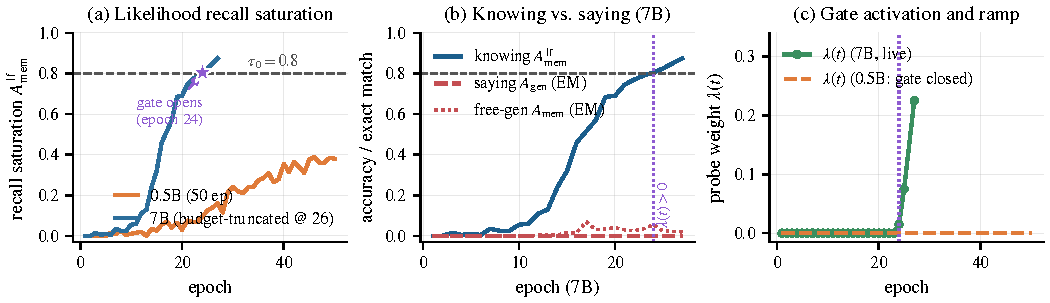
\includegraphics[width=\textwidth]{fig_saturation.pdf}
\caption{Scale-dependent saturation and live gate activation.
\textbf{(a)} Likelihood recall $\amemlf$ vs.\ epoch for both scales;
the 7B model crosses $\tau_0{=}0.8$ (dashed) at epoch 24 (star), the
0.5B model plateaus at $0.39$ after 50 epochs.
\textbf{(b)} The 7B knowing--saying dissociation: teacher-forced recall
climbs to $0.875$ while paraphrase exact match ($\agen$) remains at
$0.000$ and free-generation EM stays $\le 0.07$.
\textbf{(c)} The gate weight $\lambda(t)$: closed for the entire 0.5B
run; opened at epoch 24 at 7B with the ramp
$0.015 \to 0.075 \to 0.225$ observed over epochs 24--27 (the run was
budget-truncated before the ramp completed to $\lambda_0{=}0.3$).}
\label{fig:sat}
\end{figure*}

Because the crossing happened mid-run, the activation transient was
logged live: the gate recorded
$(\amemlf, \lambda) = (0.805, 0.015)$ at epoch 24,
$(0.825, 0.075)$ at epoch 25, and $(0.875, 0.225)$ at epoch 27
(Fig.~\ref{fig:sat}c). To our knowledge this is an unusually direct
capture of a ``memorization threshold'' crossing during a real
fine-tuning run; the ramp toward $\lambda_0{=}0.3$ was cut short by the
compute budget, so the regularized phase (probe loss flowing into the
backbone) is exercised but not yet studied at length---we return to this
in Section~\ref{sec:res:post}.

\subsection{Knowing is not saying}
\label{sec:res:gap}

Figure~\ref{fig:gap} plots the five recall/production channels for both
scales. Two dissociations are visible. First, \emph{knowing vs.\
saying}: at 7B the teacher-forced recall reaches $0.875$ while
free-generation exact match stays $\le 0.07$ and paraphrase exact match
is exactly $0.000$ at every epoch; the 0.5B model shows the same
qualitative pattern ($0.39$ vs.\ $0.025$ vs.\ $0.000$). Second,
\emph{storage vs.\ assembly}: at epoch 27 the 7B generations contain
the target string as a substring $76.5\%$ of the time while exact match
is $2\%$---the entity identity is present in the output but framed
wrong (extra tokens, wrong surface form), which is precisely the
failure mode that free-generation EM conflates with ignorance and that
the likelihood metric separates. Token-level recall ($0.987$ at 7B)
confirms that the first answer token---the identity-bearing
token---is almost always correct under forcing; what fails is the
assembly of a well-formed answer under free decoding.

\begin{figure}[t]
\centering
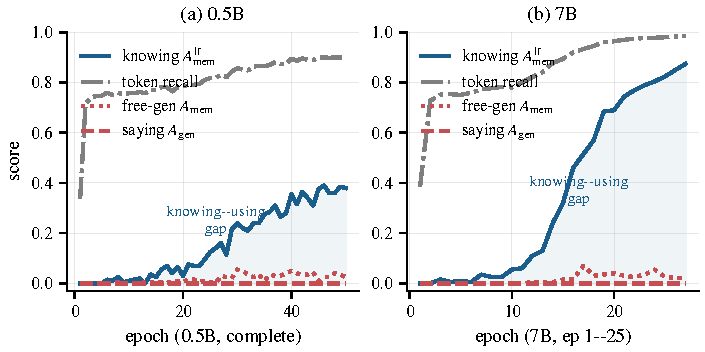
\includegraphics[width=0.80\columnwidth]{fig_knowing_saying.pdf}
\caption{Knowing vs.\ saying at both scales. Shaded region: the
knowing--using gap between teacher-forced recall and free-generation
production. Paraphrase exact match ($\agen$, dashed) never leaves zero
at either scale.}
\label{fig:gap}
\end{figure}

The knowing--using gap is thus not a delay that more epochs alone close
at small scale: the 0.5B model's gap persists through 50 epochs
($0.38$ vs.\ $0.025$), and the 7B model's gap is $0.855$ in recall
terms at the moment the gate opens. Regularization or decoding
interventions that target the \emph{saying} pathway (e.g., the
$\lambda$-gated probe loss, or answer-assembly training) are therefore
better placed than additional memorization pressure.

\subsection{Dynamics: eval reversal and bounded adaptive control}
\label{sec:res:control}

Figure~\ref{fig:dyn} shows the shared training dynamics. Held-out eval
loss bottoms at epoch 3 for both scales ($3.36$ and $3.21$) and then
rises monotonically ($4.64$ and $4.41$ by the last completed epoch)---
the memorization signature. Training loss falls from $\sim$13 to
$\sim$0.9 (0.5B) and $\sim$0.85 (7B), with the 7B run reaching lower
CE earlier ($\sim$0.30 mean by epoch 25).

\begin{figure*}[t]
\centering
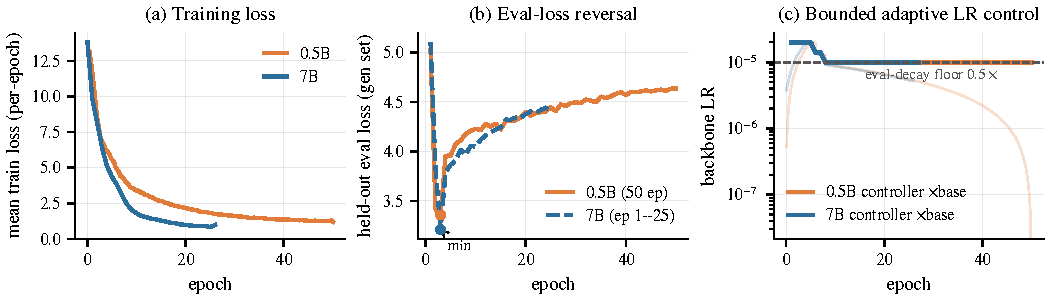
\includegraphics[width=\textwidth]{fig_dynamics.pdf}
\caption{Training dynamics. \textbf{(a)} Mean per-epoch training loss.
\textbf{(b)} Held-out eval loss reverses at epoch 3 at both scales and
rises thereafter---the memorization signature the gate waits for.
\textbf{(c)} Controller behavior: both runs decay the LR twice under
held-out divergence, then hold at the $0.5\times$ damping floor
(dashed).}
\label{fig:dyn}
\end{figure*}

The controller behaved identically at both scales: two eval-driven
decays (epochs 6 and 8; multiplier $1.0 \to 0.7 \to 0.5$) followed by
a hold at the floor for the rest of training, with plateau boosts
correctly suppressed while eval loss degraded. This is the repaired
behavior. Without the floor (pilot runs), the same controller applied
consecutive $0.7\times$ decays and drove the multiplier to $0.17$,
freezing memorization with $\amemlf$ pinned at $\sim$0.02 and making
$\tau_0$ unreachable; Appendix~\ref{app:spiral} documents the failure
and the validation sequence (unit tests plus a dedicated 5-epoch GPU
gate check) that the repair passed before these production runs.

\subsection{Probes read memorization before the model can say it}
\label{sec:res:probe}

Figure~\ref{fig:probe}a shows the probe's epoch-end accuracy on
memorized vs.\ held-out entity states. At both scales the probe
separates the two populations within a few epochs ($7$--$13\%$ vs.\
$\approx 0\%$ at chance $1/1600$), and the separation tracks the
saturation curve: at 7B the probe's memorization accuracy roughly
doubles after the gate opens. The probe loss
(Fig.~\ref{fig:probe}b) falls from chance $\ln 1600 \approx 7.38$ to
below chance by orders of magnitude---reaching $\sim$$10^{-3}$ with
$100\%$ train-batch accuracy at 7B---while remaining a pure observer
during warm-up. Two practical readings follow: the probe is a cheap
early-warning monitor (its signal is unambiguous epochs before any
behavioral metric moves), and its health is verifiable online (loss
far below chance, held-out accuracy at chance), addressing the classic
probe-reliability concern \citep{hewitt2019control}.

\begin{figure}[t]
\centering
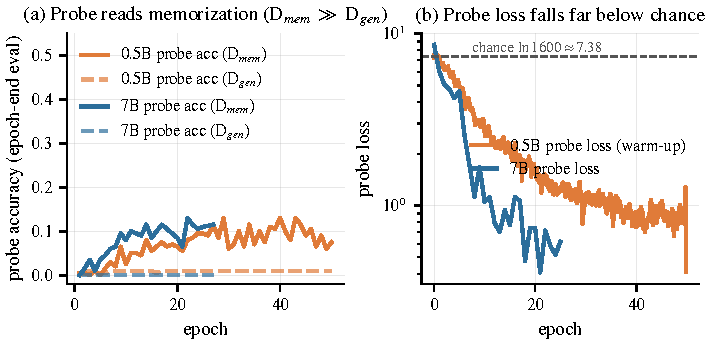
\includegraphics[width=0.82\columnwidth]{fig_probe.pdf}
\caption{Probe health. \textbf{(a)} Epoch-end probe accuracy on
memorized ($\mathcal{D}_{\mathrm{mem}}$ subsample) vs.\ held-out
($\mathcal{D}_{\mathrm{gen}}$) entity states; chance is $1/1600$.
\textbf{(b)} Probe loss (log scale) falls far below chance at both
scales during detached warm-up.}
\label{fig:probe}
\end{figure}

\subsection{Update anatomy: upper-layer MLPs carry the memorization}
\label{sec:res:anatomy}

From the released adapters we compute the effective weight update
$\Delta W = \tfrac{\alpha}{r} BA$ per adapted projection
(Fig.~\ref{fig:anat}). The pattern is consistent across scales and
consistent with the storage literature: MLP projections carry
$69.7\%$ (0.5B) and $73.3\%$ (7B) of total update mass
$\sum_l \lVert \Delta W \rVert_F$; the upper half of layers carries
$57.8\%$ and $56.1\%$; and the top three modules are
gate-, up-, and down-projection at both scales, with key/value
attention projections nearly untouched. The 7B adapter analyzed here
is the epoch-26 state, i.e., one to two epochs \emph{after} gate
activation, so the concentration is not an artifact of an
un-activated regime.

\begin{figure}[t]
\centering
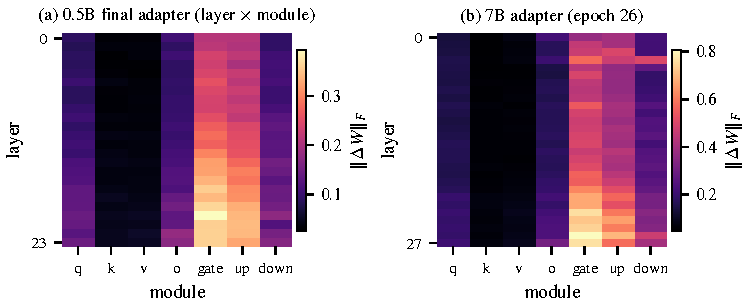
\includegraphics[width=0.78\columnwidth]{fig_anatomy.pdf}
\caption{Update anatomy $\lVert \Delta W \rVert_F$ per
(layer, module). \textbf{(a)} 0.5B final adapter (epoch 50);
\textbf{(b)} 7B adapter at epoch 26 (post-activation). MLP projections
(gate/up/down) dominate at both scales; color scales are per-panel.}
\label{fig:anat}
\end{figure}

\subsection{The regularized phase and its truncation}
\label{sec:res:post}

Honesty about scope: the gate opened at 7B only $\sim$3 epochs before
the compute budget terminated the run, so the post-activation phase
(probe loss at $\lambda$ up to $0.225$ flowing into the backbone) is
\emph{exercised and logged} but not yet studied over the tens of
epochs its design assumes. Within the observed window the phase is
stable (no loss or gradient spikes; $\amemlf$ continues to rise;
no further controller interventions). Whether the probe-regularized
phase closes the \emph{saying} gap---the motivation for the
design---remains the central open question for the completed 7B run;
the 0.5B run suggests it will not be answerable at that scale at all,
since the gate never opens there within 50 epochs.
